% 2009 年天津卷理科第 19 题：五面体 ABCDEF，FA⊥平面 ABCD，AD∥BC∥FE。
% 来源 PDF：普通高考/2009/2009天津理.pdf，SHA256 ea758271e47ecf0aadf9b6ea943bcdf2df78b8bf284c3ef26b72c4b69eeb3e80
% 原页：第 2 页（A3 三栏）第 1 栏上部，印刷页 562。
% 重绘依据：A 前左下、B 前右下、C 右后、D 左后；F 在 A 正上方，E 在 F 后上方且 FE∥AD；
%   M 为 EC 中点。被遮挡的 D-A 画虚线。
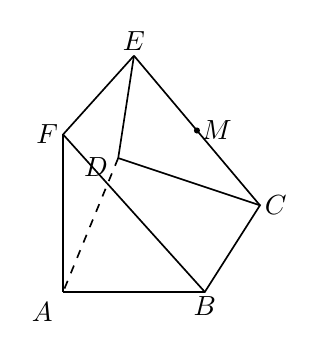
\begin{tikzpicture}[scale=1.0, semithick, every node/.style={inner sep=1.5pt}]
  \coordinate (A) at (0,0);
  \coordinate (B) at (1.8,0);
  \coordinate (C) at (2.5,1.1);
  \coordinate (D) at (0.7,1.7);
  \coordinate (F) at (0,2.0);
  \coordinate (E) at (0.9,3.0);
  \coordinate (M) at (1.7,2.05);
  % 底面
  \draw (A) -- (B) -- (C) -- (D);
  \draw[dashed] (D) -- (A);
  % 棱
  \draw (A) -- (F);
  \draw (F) -- (E);
  \draw (B) -- (F);
  \draw (C) -- (E);
  \draw (E) -- (D);
  % M
  \fill (M) circle (1.1pt);
  \node[anchor=north east] at ([xshift=-2pt,yshift=-2pt]A) {$A$};
  \node[anchor=north] at (B) {$B$};
  \node[anchor=west] at (C) {$C$};
  \node[anchor=north east] at ([xshift=-2pt,yshift=2pt]D) {$D$};
  \node[anchor=east] at (F) {$F$};
  \node[anchor=south] at (E) {$E$};
  \node[anchor=west] at (M) {$M$};
\end{tikzpicture}
